\documentclass{article}

% Numeric citations (NeurIPS allows numeric if consistent).
\PassOptionsToPackage{numbers,compress}{natbib}
\usepackage[preprint]{neurips_2024}

\usepackage[utf8]{inputenc}
\usepackage[T1]{fontenc}
\usepackage{hyperref}
\usepackage{url}
\usepackage{booktabs}
\usepackage{amsfonts}
\usepackage{nicefrac}
\usepackage{microtype}
\usepackage{xcolor}
\usepackage{graphicx}
\usepackage{amsmath,amssymb}
\usepackage{siunitx}
\usepackage{multirow}
\usepackage{tikz}
\usetikzlibrary{arrows.meta,positioning,fit,calc}

\title{Transformixer: Attention-Based Variate Mixing without Positional Bias for Multivariate Forecasting}

\author{
  Morteza Ziabakhsh\\
  University of Tehran\\
  \texttt{m.ziabakhsh@ut.ac.ir}
}

\begin{document}

\maketitle

\begin{abstract}
Multivariate long-term forecasting requires models that capture both temporal dynamics and cross-variate dependencies.
Recent mixer architectures such as xLSTM-Mixer combine an efficient shared linear temporal forecast with an xLSTM-based joint variate mixer.
However, recurrent mixing along the variate axis is inherently order-sensitive: it depends on an arbitrary channel ordering, propagates information sequentially across channels, and relies on a forward/reverse multi-view mechanism to mitigate that dependence.
We propose \textbf{Transformixer}, which retains reversible instance normalization and shared NLinear temporal mixing, but replaces the ordered sLSTM variate mixer with a Transformer encoder over variate tokens \emph{without} positional encodings.
The resulting mixer is permutation-equivariant, realizes direct pairwise interactions among all variates in a single layer, and removes the need for memory tokens and bidirectional multi-view fusion.
On Electricity and Traffic with lookback and horizon $96$, we report both the PE-free default and a fixed-sinusoidal-PE variant alongside five external baselines.
Transformixer+PE achieves the best ECL result among all compared models (MSE $0.1403$, MAE $0.2315$), while the PE-free default improves upon xLSTM-Mixer on Traffic (including the best MAE among compared models).
A controlled ablation under the same RevIN+NLinear front-end confirms that variate mixing is necessary on both datasets and that positional bias is dataset-dependent: fixed channel-position encodings help ECL but not Traffic relative to the PE-free mixer.
Our study is intentionally limited in breadth by available compute and time (two datasets, one horizon, single seeds); nevertheless, the present results suggest that Transformixer is a promising direction, and future work can explore this idea more thoroughly across additional datasets, horizons, and training budgets.
\end{abstract}

\section{Introduction}
\label{sec:intro}

Multivariate time series forecasting is central to energy, traffic, and industrial monitoring, where many correlated channels are observed jointly.
Deep models must therefore learn temporal structure \emph{and} cross-channel interactions.
Transformers~\citep{vaswani2017attention} have been widely adapted to this setting, from efficient temporal attention~\citep{zhou2021informer} and patch-based channel-independent encoders~\citep{nie2023patchtst} to inverted architectures that attend over variate tokens~\citep{liu2024itransformer}.
In parallel, strong linear and mixer baselines~\citep{zeng2023dlinear,li2023rlinear,kraus2024xlstmmixer} show that careful temporal mapping and lightweight mixing remain highly competitive.

xLSTM-Mixer~\citep{kraus2024xlstmmixer} is representative of the latter line: a shared NLinear temporal forecast is refined by an xLSTM~\citep{beck2024xlstm} (sLSTM) block that mixes information along the \emph{variate} axis, optionally with memory tokens, and reconciles forward and reversed channel views.
This design is effective, but it encodes a questionable inductive bias whenever channel indices lack a natural total order (e.g., sensors or customer meters).
Sequential mixing makes the computation depend on an arbitrary ordering, forces long-range channel interactions to travel through a recurrent state, and motivates an auxiliary reverse view to reduce order artifacts.

We ask whether a simpler, set-structured mixer is a better fit.
\textbf{Transformixer} keeps the successful temporal front-end of xLSTM-Mixer, reversible instance normalization~\citep{kim2021revin} and shared NLinear temporal mixing~\citep{zeng2023dlinear}, but replaces the sLSTM variate mixer with a Transformer encoder applied to variate tokens \emph{without} positional encodings and without a causal mask.
Beyond permutation equivariance~\citep{zaheer2017deepsets}, attention provides direct pairwise interactions among all channels, multi-head specialization, and a single forward pass that no longer needs memory tokens or bidirectional view fusion.
This view is complementary to iTransformer~\citep{liu2024itransformer}: we reuse variate-token attention as a \emph{mixer block} after an explicit temporal linear forecast, rather than as a full inverted backbone.

\paragraph{Contributions.}
\begin{itemize}
  \item We introduce Transformixer, a drop-in permutation-equivariant Transformer variate mixer for the xLSTM-Mixer pipeline.
  \item We analyze inductive-bias differences versus ordered sLSTM mixing (equivariance, global interactions, architectural simplification, and parallelism), not only forecasting accuracy.
  \item We compare against five baselines on Electricity and Traffic ($L{=}H{=}96$) and report a controlled mixer ablation (sLSTM FULL, PE-free Transformer, Transformer with fixed PE, and NLinear-only) under a shared training recipe.
  \item We discuss when the redesign helps and how the equivariance--accuracy tradeoff depends on the dataset, under clearly stated limitations.
\end{itemize}

\section{Related Work}
\label{sec:related}

\paragraph{Transformer architectures for long-term forecasting.}
The Transformer~\citep{vaswani2017attention} has become a dominant backbone for long-term time series forecasting (LTSF), motivating a line of work that adapts attention to long horizons and non-stationary signals.
Informer~\citep{zhou2021informer} reduces the cost of canonical self-attention with ProbSparse attention and a generative decoder, enabling longer lookbacks than early encoder--decoder designs.
Autoformer~\citep{wu2021autoformer} embeds seasonal--trend decomposition into the network and replaces standard attention with an auto-correlation mechanism that emphasizes period-based dependencies.
FEDformer~\citep{zhou2022fedformer} further couples decomposition with frequency-domain attention, arguing that sparse spectral representations capture global structure more effectively than purely temporal attention.
Subsequent models broaden the representational toolkit: TimesNet~\citep{wu2023timesnet} reshapes 1D series into 2D tensors to model intra- and inter-period variation, while PatchTST~\citep{nie2023patchtst} segments each univariate channel into patches and applies a channel-independent Transformer, often matching or exceeding heavier multivariate attention models on standard LTSF benchmarks.
These works primarily innovate on \emph{temporal} representation and efficiency; cross-variate interaction, when present, is typically entangled with time-axis attention rather than isolated as an explicit mixer.

\paragraph{Channel independence versus cross-variate modeling.}
A recurring design tension in multivariate forecasting is whether channels should be modeled independently or jointly.
Channel-independent approaches such as PatchTST~\citep{nie2023patchtst} and strong linear baselines~\citep{zeng2023dlinear,li2023rlinear} share temporal parameters across variates but avoid explicit cross-channel mixing, which can improve robustness when inter-variate relations are weak or unstable.
In contrast, several Transformers target cross-dimension dependency directly.
Crossformer~\citep{zhang2023crossformer} uses dimension-segment-wise embeddings and two-stage attention to capture cross-time and cross-dimension interactions hierarchically.
iTransformer~\citep{liu2024itransformer} inverts the conventional layout: each variate's full series becomes a token, so attention mixes channels while feed-forward layers process series representations.
This inverted view is closely related to Transformixer's variate-token mixer; the difference is architectural placement.
iTransformer is a full inverted backbone, whereas Transformixer applies PE-free attention as a \emph{drop-in variate mixer} after an explicit shared NLinear temporal forecast inside a mixer-style pipeline.

\paragraph{Linear models and MLP mixers.}
Challenging the necessity of deep temporal attention, LTSF-Linear / DLinear / NLinear~\citep{zeng2023dlinear} show that simple linear maps, especially with last-value normalization, can rival Transformers on many benchmarks.
RLinear~\citep{li2023rlinear} revisits linear mapping with RevIN-style normalization and reinforces that carefully normalized linear temporal projections remain highly competitive.
Building on MLP-Mixer ideas from vision, TSMixer~\citep{chen2023tsmixer} alternates time-mixing and feature-mixing MLP blocks to capture temporal and cross-variate structure with favorable parameter scaling.
TimeMixer~\citep{wang2024timemixer} extends mixing to multiple temporal resolutions via past decomposable mixing and future multipredictor mixing.
Collectively, these results motivate hybrid designs that keep an efficient temporal front-end and allocate capacity where cross-variate reasoning is needed, the regime in which xLSTM-Mixer and Transformixer operate.

\paragraph{Recurrent mixers and xLSTM.}
Despite the Transformer wave, recurrent models have regained attention through xLSTM~\citep{beck2024xlstm}, which revisits LSTM-style memory with exponential gating and enriched memory structures (including scalar sLSTM blocks).
xLSTM-Mixer~\citep{kraus2024xlstmmixer} instantiates this idea for multivariate forecasting: a shared linear (NLinear) temporal forecast is refined by sLSTM blocks that mix along the variate axis, optionally with memory tokens, and reconcile forward and reversed channel views.
The design demonstrates that recurrent joint mixing can be state-of-the-art, but it also inherits order sensitivity along channels and relies on multi-view fusion to mitigate arbitrary variate orderings.
Transformixer keeps the RevIN + NLinear temporal pathway of this lineage while replacing the ordered sLSTM mixer with set-structured self-attention.

\paragraph{Normalization and set inductive biases.}
Non-stationarity is a central obstacle in LTSF.
RevIN~\citep{kim2021revin} applies reversible instance normalization to reduce distribution shift between train and test windows and is now a standard component in many competitive models, including both xLSTM-Mixer and Transformixer.
Separately, set learning theory~\citep{zaheer2017deepsets} formalizes permutation-invariant and equivariant maps over unordered collections.
When multivariate channels lack a natural total order, as with sensors, meters, or traffic detectors, treating variates as a set is a natural inductive bias.
Transformixer's default omission of positional encodings along the variate axis is a concrete realization of that principle: the mixer is permutation-equivariant by construction, in contrast to recurrent ordered mixing and to Transformer mixers that inject positional signals on the channel axis.
Our ablation results (Section~\ref{sec:ablation}) show that this design choice is not uniformly optimal in accuracy, motivating future work on learnable channel orderings.

\paragraph{Positioning.}
In summary, prior work offers strong temporal Transformers, channel-independent patch models, linear and MLP mixers, inverted variate-token attention, and recurrent joint mixers.
Transformixer sits at their intersection: it inherits an efficient linear temporal forecast from the mixer/linear literature, adopts variate-token attention in the spirit of iTransformer, and specifically targets the order-sensitive bottleneck of xLSTM-Mixer's sLSTM variate stage with a PE-free, single-view Transformer mixer.

\section{Method}
\label{sec:method}

\subsection{Problem setup}
Given a lookback window $X \in \mathbb{R}^{L \times C}$ with $C$ variates, the goal is to predict the future horizon $Y \in \mathbb{R}^{H \times C}$.
We consider multivariate-to-multivariate forecasting.
Transformixer implements a map $f_\theta: \mathbb{R}^{L \times C} \rightarrow \mathbb{R}^{H \times C}$ composed of normalization, temporal mixing, equivariant variate mixing, and denormalization (Figure~\ref{fig:arch}).

\begin{figure}[t]
  \centering
  \resizebox{0.98\linewidth}{!}{%
  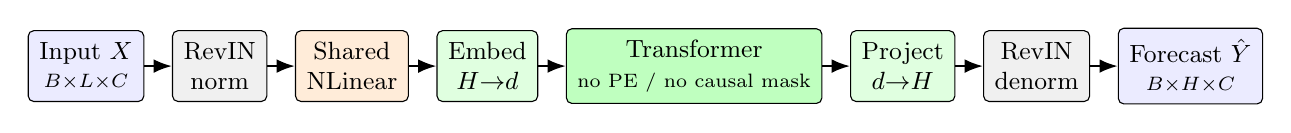
\begin{tikzpicture}[
    font=\small,
    box/.style={draw, rounded corners=2pt, align=center, inner sep=4pt, minimum height=9mm},
    arrow/.style={-{Latex}, thick}
  ]
    \node[box, fill=blue!8] (in) {Input $X$\\[-1pt]{\scriptsize $B{\times}L{\times}C$}};
    \node[box, fill=gray!12, right=0.35cm of in] (revin) {RevIN\\norm};
    \node[box, fill=orange!15, right=0.35cm of revin] (nlin) {Shared\\NLinear};
    \node[box, fill=green!12, right=0.35cm of nlin] (emb) {Embed\\$H{\rightarrow}d$};
    \node[box, fill=green!25, right=0.35cm of emb] (tr) {Transformer\\{\scriptsize no PE / no causal mask}};
    \node[box, fill=green!12, right=0.35cm of tr] (fc) {Project\\$d{\rightarrow}H$};
    \node[box, fill=gray!12, right=0.35cm of fc] (den) {RevIN\\denorm};
    \node[box, fill=blue!8, right=0.35cm of den] (out) {Forecast $\hat Y$\\[-1pt]{\scriptsize $B{\times}H{\times}C$}};
    \foreach \a/\b in {in/revin,revin/nlin,nlin/emb,emb/tr,tr/fc,fc/den,den/out}
      \draw[arrow] (\a) -- (\b);
  \end{tikzpicture}}
  \caption{Transformixer overview. Temporal structure is handled by shared NLinear; cross-variate structure is handled by a PE-free Transformer over variate tokens.}
  \label{fig:arch}
\end{figure}

\subsection{Reversible instance normalization}
Following~\citet{kim2021revin}, we apply RevIN with non-affine statistics along the temporal axis of each variate, normalize the lookback window, and denormalize the forecast at the end of the network.
This reduces sensitivity to non-stationarity without altering the mixer design.

\subsection{Shared NLinear temporal mixing}
Let $x \in \mathbb{R}^{B \times L \times C}$ denote the RevIN-normalized batch.
We use the NLinear residual map of~\citet{zeng2023dlinear}: subtract the last observed value, apply a linear layer shared across channels that maps length $L$ to horizon $H$, then add the last value back,
\begin{equation}
  \hat Y_0
  =
  \mathrm{Linear}_{L \rightarrow H}\!\bigl(x - x_{:,-1,:}\bigr) + x_{:,-1,:},
\end{equation}
yielding a preliminary forecast $\hat Y_0 \in \mathbb{R}^{B \times H \times C}$.
This stage models temporal dynamics efficiently and independently of channel order.

\subsection{Variate tokenization and Transformer mixing}
We rearrange $\hat Y_0$ so that each variate becomes a token of dimension $H$, embed tokens with a linear map $H \rightarrow d$, and process the sequence of $C$ tokens with a stack of standard Transformer encoder layers~\citep{vaswani2017attention}: multi-head self-attention and a position-wise feed-forward network, with residual connections and layer normalization.
Crucially, the default model \emph{omits positional encodings} and uses full (non-causal) attention.
Our implementation also supports an optional fixed sinusoidal positional embedding on the variate axis for ablation; adding PE breaks permutation equivariance.
A final linear map $d \rightarrow H$ produces refined horizon vectors per variate, which are rearranged and RevIN-denormalized to obtain $\hat Y$.

\paragraph{Permutation equivariance (PE-free default).}
When positional encodings are omitted, the embedding, attention, feed-forward maps, and output projection are applied identically to every token and attention is a symmetric function of the token set, so for any channel permutation matrix $P$,
\begin{equation}
  f_\theta(XP) = f_\theta(X)P.
\end{equation}
Thus the model treats variates as a set rather than an ordered sequence.
We verify this property with a dedicated unit test in our implementation.

\subsection{Design rationale versus xLSTM-Mixer}
\label{sec:rationale}
Table~\ref{tab:diff} summarizes what Transformixer keeps and removes.
Beyond equivariance, replacing sLSTM with attention is motivated by several inductive biases:

\begin{enumerate}
  \item \textbf{Direct global interactions.}
  Self-attention couples every pair of variates in one layer ($O(1)$ path length over channels).
  An sLSTM mixes channels sequentially, so information from channel $i$ to $j$ must travel through the recurrent state (and/or a small set of memory tokens), with path length depending on an arbitrary ordering.
  This distinction is especially relevant for high-$C$ series such as Traffic ($C{=}862$).

  \item \textbf{Multi-head specialization.}
  Different heads can learn distinct dependency patterns in parallel, whereas a single recurrent state stream is less naturally factored into multiple interaction types.

  \item \textbf{Architectural simplification.}
  Order-agnostic mixing removes the need for xLSTM-Mixer's forward/reverse multi-view fusion and for auxiliary memory tokens.
  Transformixer uses a single forward pass over variate tokens.

  \item \textbf{Hardware-parallel mixing.}
  Attention is token-parallel over $C$, whereas recurrence is sequential in $C$.
  We do \emph{not} claim wall-clock superiority: attention costs $O(C^2 d)$ per layer and may become expensive for very large $C$.
\end{enumerate}

\begin{table}[t]
  \centering
  \caption{Transformixer versus xLSTM-Mixer (FULL setting used in our runs).}
  \label{tab:diff}
  \begin{tabular}{lcc}
    \toprule
    Component & xLSTM-Mixer & Transformixer \\
    \midrule
    RevIN & yes & yes \\
    Shared NLinear temporal mix & yes & yes \\
    Variate mixer & sLSTM (+ mem.\ tokens) & Transformer encoder \\
    Positional encoding on variates & n/a (order via recurrence) & none \\
    Forward/reverse multi-view & yes & no \\
    Memory tokens & yes (3 in our runs) & no \\
    \bottomrule
  \end{tabular}
\end{table}

\section{Experimental Setup}
\label{sec:setup}

\paragraph{Datasets.}
We evaluate on two standard multivariate benchmarks commonly used in long-term forecasting~\citep{zhou2021informer,wu2021autoformer}:
\textbf{Electricity} (ECL; $C{=}321$ hourly client loads) and \textbf{Traffic} ($C{=}862$ hourly road occupancy rates).
Following common practice, we use a chronological $70\%/10\%/20\%$ train/validation/test split and fit a StandardScaler on the training portion only.

\paragraph{Protocol.}
All models use lookback $L{=}96$ and prediction horizon $H{=}96$ in the multivariate setting.
We report mean squared error (MSE) and mean absolute error (MAE) on the denormalized forecasts.
We compare Transformixer to five baselines that we re-ran in the same project setting: RLinear~\citep{li2023rlinear}, Informer~\citep{zhou2021informer}, PatchTST~\citep{nie2023patchtst}, iTransformer~\citep{liu2024itransformer}, and xLSTM-Mixer~\citep{kraus2024xlstmmixer}.

\paragraph{Training details.}
Transformixer and xLSTM-Mixer are trained with Adam, learning rate $5{\times}10^{-4}$, batch size $32$, L1 loss, and up to $10$ epochs with a warmup--cosine schedule (seed $42$).
Both use embedding width $1024$, $16$ heads, and $2$ mixer blocks/layers with dropout $0.1$.
For each baseline, we follow the hyperparameters recommended by the authors of the corresponding paper (or the accompanying official codebase) for the given dataset setting, including model width, depth, learning rate, and related training choices where applicable.
In contrast, Transformixer does \emph{not} benefit from a dedicated hyperparameter search: its architectural and optimization settings are largely inherited from the xLSTM-Mixer experimental scripts rather than tuned specifically for the Transformer mixer.
The baselines therefore enjoy published, author-recommended configurations, while Transformixer is evaluated under a comparatively untuned setup.
We treat the study as an architectural comparison under practical training budgets rather than a fully unified or exhaustively tuned hyperparameter sweep.

\paragraph{Controlled mixer ablation.}
To isolate the effect of the variate mixer while keeping the temporal front-end fixed, we retrain four variants under the same recipe above: (A) NLinear-only (RevIN+NLinear with the mixer disabled), (B) xLSTM-Mixer FULL (sLSTM with memory tokens and forward/reverse fusion), (C) Transformixer without PE (our default), and (D) Transformixer with fixed sinusoidal PE on variate tokens.
Table~\ref{tab:main} reports both Transformixer variants---PE-free (C) and fixed-PE (D)---alongside external baselines; Table~\ref{tab:ablation} summarizes the full controlled comparison.

\paragraph{Scope limitations.}
Due to limited computational resources and project time, we report a single run per model--dataset pair, only horizon $96$, and only two datasets.
We do not claim comprehensive state-of-the-art coverage; broader multi-horizon and multi-seed evaluation is left to future work (Section~\ref{sec:discussion}).

\section{Results}
\label{sec:results}

\begin{table}[t]
  \centering
  \caption{Forecasting results for lookback/horizon $96$. Best is \textbf{bold}; second-best is \underline{underlined}.}
  \label{tab:main}
  \setlength{\tabcolsep}{4pt}
  \begin{tabular}{lcccc}
    \toprule
    & \multicolumn{2}{c}{ECL} & \multicolumn{2}{c}{Traffic} \\
    \cmidrule(lr){2-3}\cmidrule(lr){4-5}
    Model & MSE & MAE & MSE & MAE \\
    \midrule
    RLinear      & 0.1973 & 0.2740 & 0.6463 & 0.3844 \\
    Informer     & 0.3263 & 0.4068 & 1.0140 & 0.5624 \\
    PatchTST     & 0.1754 & 0.2603 & 0.4699 & 0.3005 \\
    iTransformer & 0.1481 & 0.2398 & \textbf{0.3931} & 0.2687 \\
    xLSTM-Mixer  & \underline{0.1480} & \underline{0.2352} & 0.4157 & \underline{0.2607} \\
    Transformixer & 0.1517 & 0.2364 & \underline{0.4068} & \textbf{0.2558} \\
    Transformixer+PE & \textbf{0.1403} & \textbf{0.2315} & 0.4152 & 0.2639 \\
    \bottomrule
  \end{tabular}
\end{table}

Table~\ref{tab:main} and Figure~\ref{fig:bars} summarize the main comparison against external baselines.
We report two Transformixer variants: the PE-free default (C) and fixed-sinusoidal PE (D); neither dominates every cell, and the better choice is dataset-dependent.

On \textbf{Traffic}, the PE-free default improves upon its direct predecessor xLSTM-Mixer on both MSE ($0.4068$ vs.\ $0.4157$) and MAE ($0.2558$ vs.\ $0.2607$), achieving the best MAE among all compared models and the second-best MSE after iTransformer.
Transformixer+PE is slightly worse on Traffic (MSE $0.4152$, MAE $0.2639$), consistent with the hypothesis that index-aware positional bias is not helpful when many channels interact without a meaningful 1-D order.

On \textbf{ECL}, Transformixer+PE leads the comparison (MSE $0.1403$, MAE $0.2315$), improving upon xLSTM-Mixer by $\approx$5.2\% relative MSE and upon the PE-free default by $\approx$7.6\% relative MSE.
The PE-free default remains slightly behind xLSTM-Mixer and iTransformer (MSE $0.1517$ vs.\ $0.1480$ / $0.1481$; $\approx 2.5\%$ relative MSE versus xLSTM-Mixer), indicating that the ECL gap of the equivariant variant is not due to attention being inherently weaker than ordered sLSTM mixing.

Weaker baselines (Informer, RLinear) lag substantially on both datasets, indicating that the evaluation setting is non-trivial and that the stronger inverted/mixer models form a meaningful comparison group.
Relative to xLSTM-Mixer, the Transformixer family trades a dataset-dependent positional-bias choice for gains on at least one benchmark per variant (Figure~\ref{fig:relative}).

\begin{figure}[t]
  \centering
  \begin{minipage}{0.98\linewidth}
    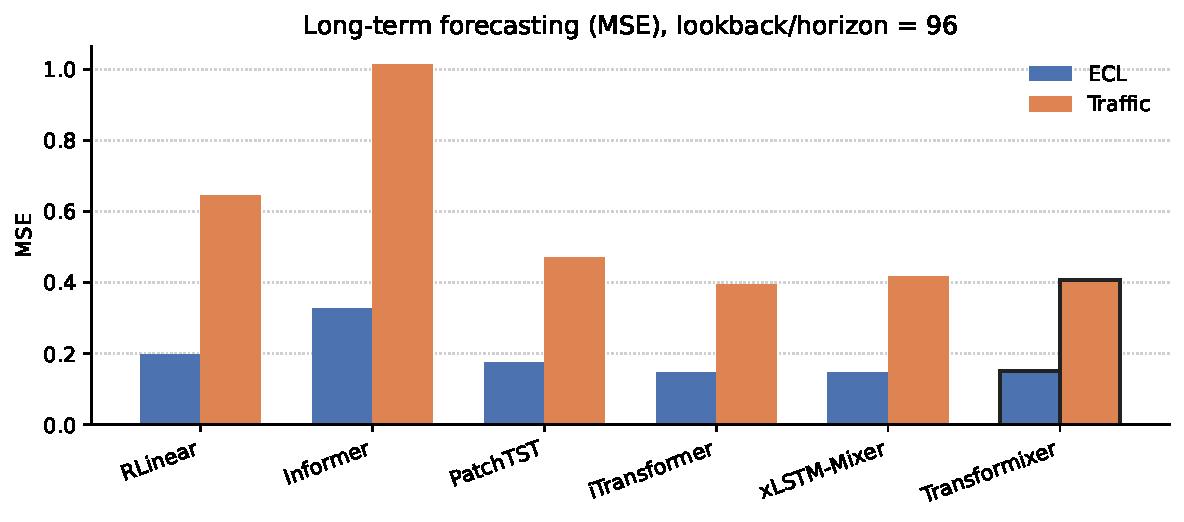
\includegraphics[width=\linewidth]{figures/results_mse.pdf}
  \end{minipage}\\[0.4em]
  \begin{minipage}{0.98\linewidth}
    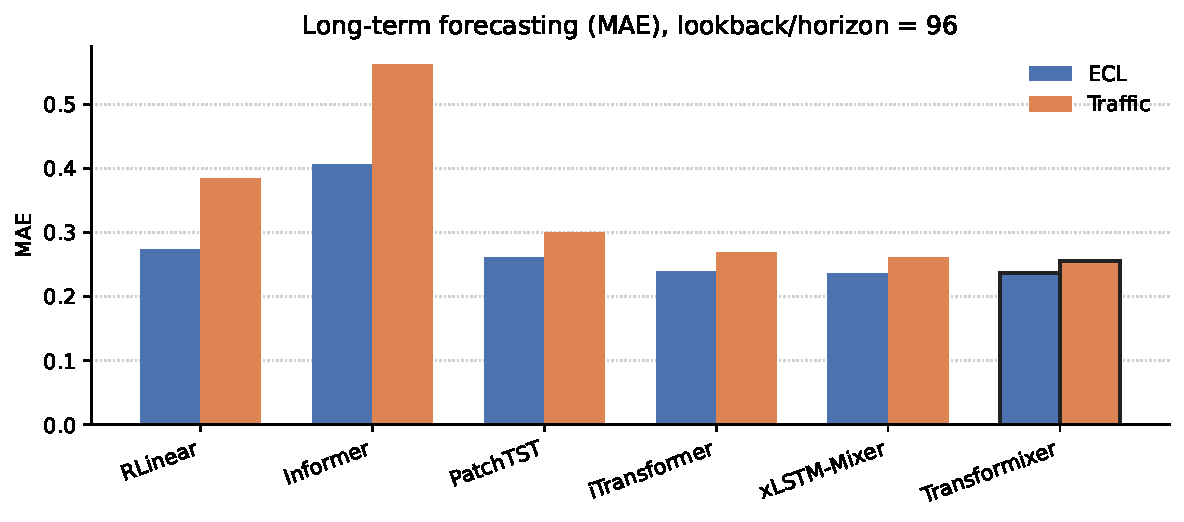
\includegraphics[width=\linewidth]{figures/results_mae.pdf}
  \end{minipage}
  \caption{MSE (top) and MAE (bottom) on ECL and Traffic ($L{=}H{=}96$). Informer omitted for scale (see Table~\ref{tab:main}); y-axes zoomed around competitive models. Both Transformixer variants are outlined.}
  \label{fig:bars}
\end{figure}

\begin{figure}[t]
  \centering
  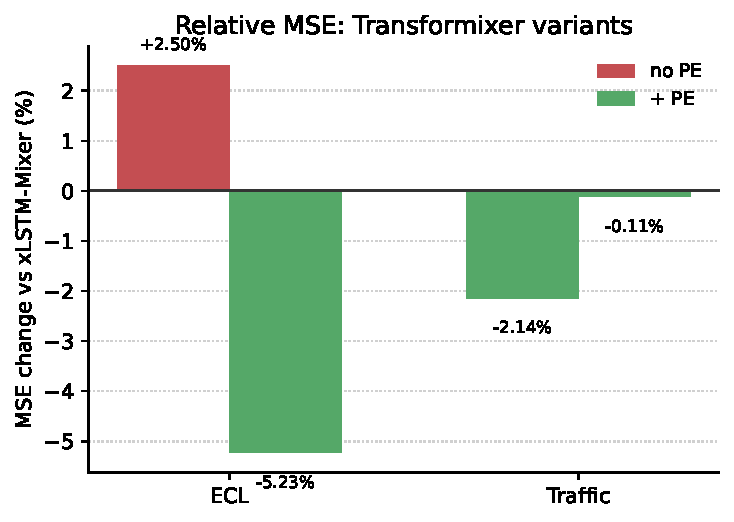
\includegraphics[width=0.55\linewidth]{figures/relative_mse_vs_xlstm.pdf}
  \caption{Relative MSE change of both Transformixer variants versus xLSTM-Mixer (negative is better for Transformixer).}
  \label{fig:relative}
\end{figure}

\subsection{Mixer ablation}
\label{sec:ablation}

Table~\ref{tab:ablation} and Figure~\ref{fig:ablation} report the controlled comparison under the shared RevIN+NLinear front-end (seed $42$, $10$ epochs, $L{=}H{=}96$).
All mixer variants substantially outperform NLinear-only (A), reducing MSE by $\approx$25--30\% on ECL and $\approx$38--39\% on Traffic, confirming that cross-variate mixing is necessary beyond shared temporal linear mapping on both benchmarks.

On \textbf{Traffic}, the PE-free default (C) is the strongest ablation variant, improving upon xLSTM FULL (B) by $\approx$2.1\% relative MSE and $\approx$1.9\% relative MAE.
Adding fixed sinusoidal PE (D) slightly degrades Traffic performance ($+2.1\%$ MSE, $+3.2\%$ MAE versus C), suggesting that index-aware positional bias is not helpful on this high-$C$ benchmark under our protocol.

On \textbf{ECL}, the pattern reverses: fixed PE (D) achieves the best ablation result (MSE $0.1403$, MAE $0.2315$), improving upon xLSTM FULL by $\approx$5.2\% relative MSE and upon the PE-free default by $\approx$7.6\% relative MSE.
This indicates that the dataset channel index carries exploitable structure on ECL, even though our experiment cannot distinguish semantic ordering, channel identity, correlation structure, or optimization effects.
Importantly, the large gain over NLinear-only on ECL shows that cross-variate mixing remains valuable there; the open question is whether positional bias should be fixed, learned, or omitted.

\begin{table}[t]
  \centering
  \caption{Controlled mixer ablation under a shared RevIN+NLinear front-end ($L{=}H{=}96$, seed $42$, $10$ epochs). Best is \textbf{bold}; second-best is \underline{underlined}.}
  \label{tab:ablation}
  \setlength{\tabcolsep}{3.5pt}
  \begin{tabular}{lcccc}
    \toprule
    & \multicolumn{2}{c}{ECL} & \multicolumn{2}{c}{Traffic} \\
    \cmidrule(lr){2-3}\cmidrule(lr){4-5}
    Variate mixer & MSE & MAE & MSE & MAE \\
    \midrule
    A: NLinear only          & 0.2016 & 0.2731 & 0.6713 & 0.3776 \\
    B: xLSTM FULL           & \underline{0.1480} & \underline{0.2352} & 0.4157 & \underline{0.2607} \\
    C: Transformixer (no PE) & 0.1517 & 0.2364 & \textbf{0.4068} & \textbf{0.2558} \\
    D: Transformixer (+ PE)  & \textbf{0.1403} & \textbf{0.2315} & \underline{0.4152} & 0.2639 \\
    \bottomrule
  \end{tabular}
\end{table}

\begin{figure}[t]
  \centering
  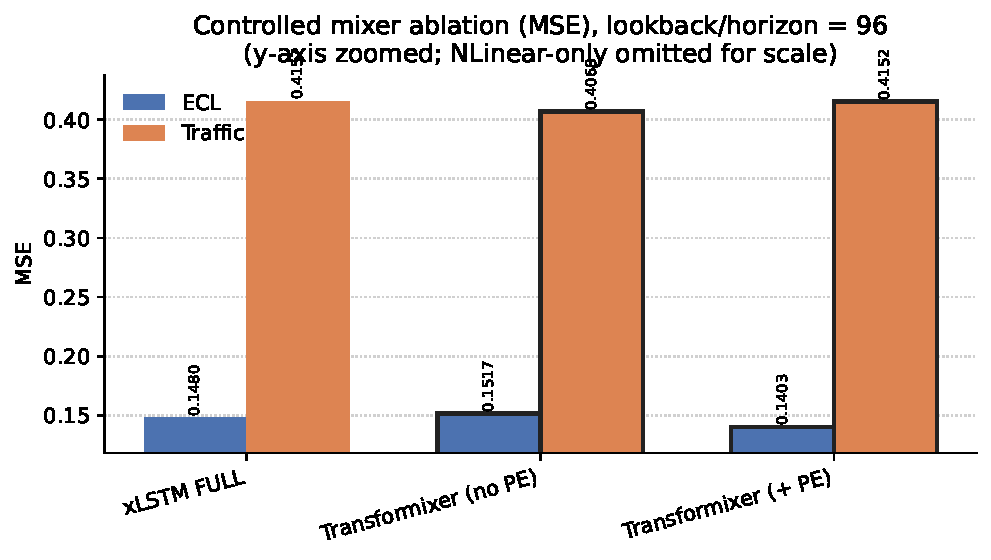
\includegraphics[width=0.98\linewidth]{figures/ablation_mse.pdf}
  \caption{Controlled mixer ablation (MSE) on ECL and Traffic. NLinear-only (A) omitted for scale (see Table~\ref{tab:ablation}); y-axis zoomed around mixer variants. Both Transformixer variants are outlined.}
  \label{fig:ablation}
\end{figure}

\subsection{Permutation behavior}
\label{sec:perm}
By construction, the PE-free default is permutation-equivariant along channels: for a channel permutation matrix $P$, $f(XP)=f(X)P$.
Unit tests in our implementation confirm this identity up to numerical tolerance; the PE ablation variant (C) does not satisfy this property.
In contrast, xLSTM-Mixer's sLSTM mixer consumes an ordered sequence of variate tokens (with an optional reverse view), so the computation itself depends on channel order.

To probe the practical effect of this distinction, we load Traffic-trained checkpoints for the PE-free default (C) and xLSTM-Mixer (B) and evaluate MSE/MAE under the identity channel order and $K{=}8$ independent random permutations of the variate axis (Table~\ref{tab:perm}).
Transformixer's errors are essentially unchanged across permutations (MSE std $1.4{\times}10^{-3}$), as expected from equivariance.
xLSTM-Mixer shows similarly small metric drift (MSE std $1.5{\times}10^{-3}$), consistent with forward/reverse multi-view partially mitigating order artifacts, but remains strictly worse on every run: mean MSE $1.349$ vs.\ $1.286$ ($\approx 4.6\%$ relative) and mean MAE $0.923$ vs.\ $0.903$ ($\approx 2.2\%$ relative).
The table makes the comparison explicit: both models are fairly stable under channel shuffles in this probe, yet Transformixer occupies a clearly better error regime without relying on ordered mixing.

Figure~\ref{fig:attn} visualizes a Transformixer attention map (first head, $64$-variate subset) from the same Traffic checkpoint.
The weights are sparse and non-uniform: a small number of key variates attract attention from many queries, indicating structured cross-variate interactions rather than uniform or purely diagonal self-attention.
This qualitative pattern aligns with the claim that the mixer models direct pairwise dependencies among channels.

\begin{table}[t]
  \centering
  \caption{Permutation probe with Traffic-trained checkpoints: identity order versus summary over the identity and $K{=}8$ random channel permutations.
  Lower is better. Transformixer is nearly invariant and consistently more accurate.}
  \label{tab:perm}
  \setlength{\tabcolsep}{4pt}
  \begin{tabular}{lcccc}
    \toprule
    & \multicolumn{2}{c}{Identity} & \multicolumn{2}{c}{Over $9$ orders (mean$\pm$std)} \\
    \cmidrule(lr){2-3}\cmidrule(lr){4-5}
    Model & MSE & MAE & MSE & MAE \\
    \midrule
    xLSTM-Mixer   & 1.3463 & 0.9224 & $1.3486{\pm}0.0015$ & $0.9233{\pm}0.0005$ \\
    Transformixer & 1.2841 & 0.9019 & $1.2865{\pm}0.0014$ & $0.9027{\pm}0.0005$ \\
    \bottomrule
  \end{tabular}
\end{table}

\begin{figure}[t]
  \centering
  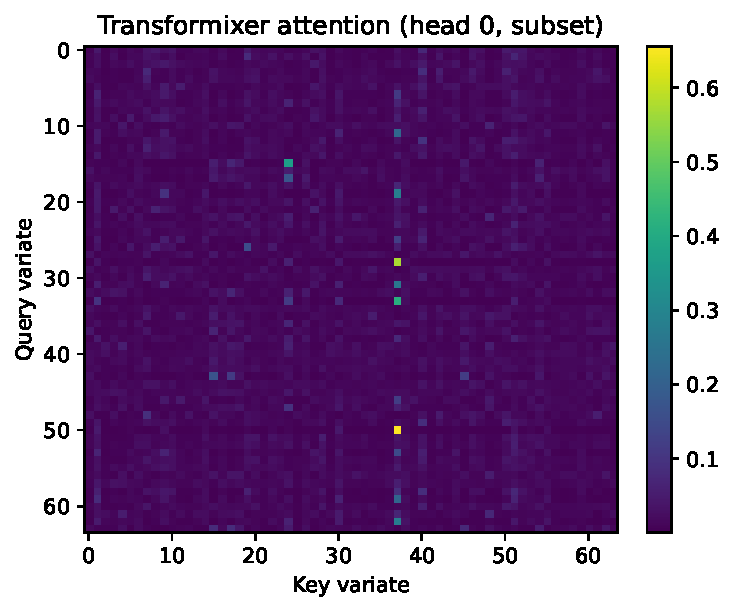
\includegraphics[width=0.55\linewidth]{figures/attention_heatmap.pdf}
  \caption{Transformixer attention weights (head~$0$) on a $64$-variate subset from a Traffic-trained model.
  Bright columns indicate key variates attended to by many queries.}
  \label{fig:attn}
\end{figure}

\section{Discussion}
\label{sec:discussion}

\paragraph{When does the Transformer mixer help?}
The Traffic improvement of the PE-free default aligns with the motivation in Section~\ref{sec:rationale}: high-$C$ forecasting benefits from direct pairwise mixing, and both the main table and ablation show that the equivariant variant is strongest on this benchmark.
The permutation probe in Section~\ref{sec:perm} further shows that the PE-free model remains stable under channel shuffles and consistently outperforms xLSTM-Mixer on that controlled evaluation, while the attention map illustrates structured cross-variate interactions.

On ECL, the story is more nuanced.
Transformixer+PE leads the main comparison and the ablation, improving upon xLSTM FULL, whereas the PE-free default trails slightly.
This cautions against a universal claim that set-structured mixing is strictly superior or inferior to ordered recurrent mixing; instead, the appropriate inductive bias appears dataset-dependent.
The ECL PE gain suggests that index-aware structure can be useful even when channels are not known to follow a semantically meaningful order, although our experiment cannot isolate the underlying mechanism.

\paragraph{Complexity tradeoff.}
Attention is more hardware-parallel over channels but asymptotically quadratic in $C$.
We did not profile latency or FLOPs in this study; efficiency claims would require dedicated measurement.
For extremely large $C$, sparse or linearized attention could be a natural extension.

\paragraph{Threats to validity.}
Results are based on single seeds, one horizon, and two datasets.
Training recipes are not fully homogenized across baseline families (loss, early stopping, seeds).
More importantly for fairness, the baselines are run with author-recommended hyperparameters, whereas Transformixer was not independently tuned and largely reuses xLSTM-Mixer settings.
This asymmetry may understate Transformixer's potential relative to well-tuned baselines.
These factors limit statistical strength and strict comparability; we report them explicitly because the project was constrained by compute and time.

\paragraph{Future work.}
A fuller evaluation would include horizons $\{96,192,336,720\}$, additional datasets (e.g., ETT, Weather), multi-seed mean$\pm$std, ablations over mixer depth and head count, and efficiency profiling.
Motivated by the dataset-dependent PE results, an appealing direction is to learn a global channel permutation or soft ordering jointly with the mixer via a differentiable relaxation such as Gumbel-Sinkhorn or differentiable sorting, allowing the model to discover an index-aware layout when it helps without committing to a fixed arbitrary order a priori.
Such experiments are feasible with additional GPU resources but were out of scope here.

\section{Conclusion}
\label{sec:conclusion}

Transformixer replaces the order-sensitive sLSTM variate mixer in xLSTM-Mixer with a PE-free Transformer over variate tokens, preserving RevIN and shared NLinear temporal mixing.
The redesign targets permutation equivariance, direct multi-head interactions, and a simpler single-view architecture without memory tokens.
Empirically, under a limited protocol, Transformixer+PE achieves the best ECL result among compared models, while the PE-free default improves on xLSTM-Mixer for Traffic.
The controlled ablation further shows that variate mixing is necessary on both datasets and that positional bias is not uniformly beneficial: fixed PE helps ECL but hurts Traffic relative to the equivariant default.
We view the contribution as an architectural study with transparent resource limits, and as evidence that mixer design should be chosen according to dataset-specific structure rather than a single universal channel-ordering assumption.

\begin{ack}
This work was conducted as a university research project under constrained computational resources and time.
Experiments were run using cloud GPU notebooks (Google Colab).
We thank the authors of the baseline codebases and benchmark datasets used in this study.
\end{ack}

\bibliographystyle{unsrtnat}
\bibliography{references}

\end{document}
